\chapter{Review against plan}

% plan produced as part of the specification, showing what has been completed, and progress to date

% any changes to the plan should be indicated
% - not adding binary search tree
% - including human testers for the evaluation phase
% - adding the settings feature

Admittedly, there are a few changes that had deviated slightly from the specification document. One of the minor changes I have made is the exclusion of adding a binary search tree from the list of animations available the program. This is mainly to ensure that I have enough time to implement the animations for other algorithms that had been mentioned in the design chapter, under the \textit{Algorithm animation designs} section (refer to section \ref{sec:algorithmAnimationDesign} on page \pageref{sec:algorithmAnimationDesign} for the list of animation designs).

Another change that I decided to make, is to include human testers to conduct the assessment of the \textit{Algorithm Animation Program}. I believe that there is a need for me to include external parties to assess and review my product, instead of doing it myself, as specified in the specification documentation. Reason being that having someone who has a different level of knowledge and understanding in this topic to test this product, would provide me with better feedback, from their point of view, about what is good or lacking in the program. For more information about the evaluation testing, do have a look at section \ref{sec:evaluationDesign} on page \pageref{sec:evaluationDesign} for more information such as, what kinds of testers that is needed, and the sets of questions and tests that will be conducted in order to make the product ideal for use.

Finally, it is worth mentioning that I have decided to add one extra feature, the \textit{settings} feature, as I believe that this will enhance the user experience when allowing the users to work on an environment that they are most comfortable in. For now, the plans only to include in changing the font size and the speed of animation due to the time constraints that was given to me. However, I am planning to implement the settings feature that would easily allow the developers to add additional features that can be changeable, thus making the program more customisable in result, in possible further iterations of the program.

\section{Updated Gantt Chart}
In the following page shows the revised version of the Gantt Chart. It has been changed slightly to fit the plans that I have devised and documented within this design documentation. What has been predominantly change is the testing phase, which is brought much forward, and now currently aligned with the implementation stage. Of course, the testing phase is expected to require a longer time compared to the implementation, as I have set ample amount of time for the testing phase. I believe that this is one of the most important phase for me to invest on and ensure that the software will be in tip top condition before the submission.

\begin{landscape}
\begin{figure}[H]
\centering
\hspace*{-0.5cm}
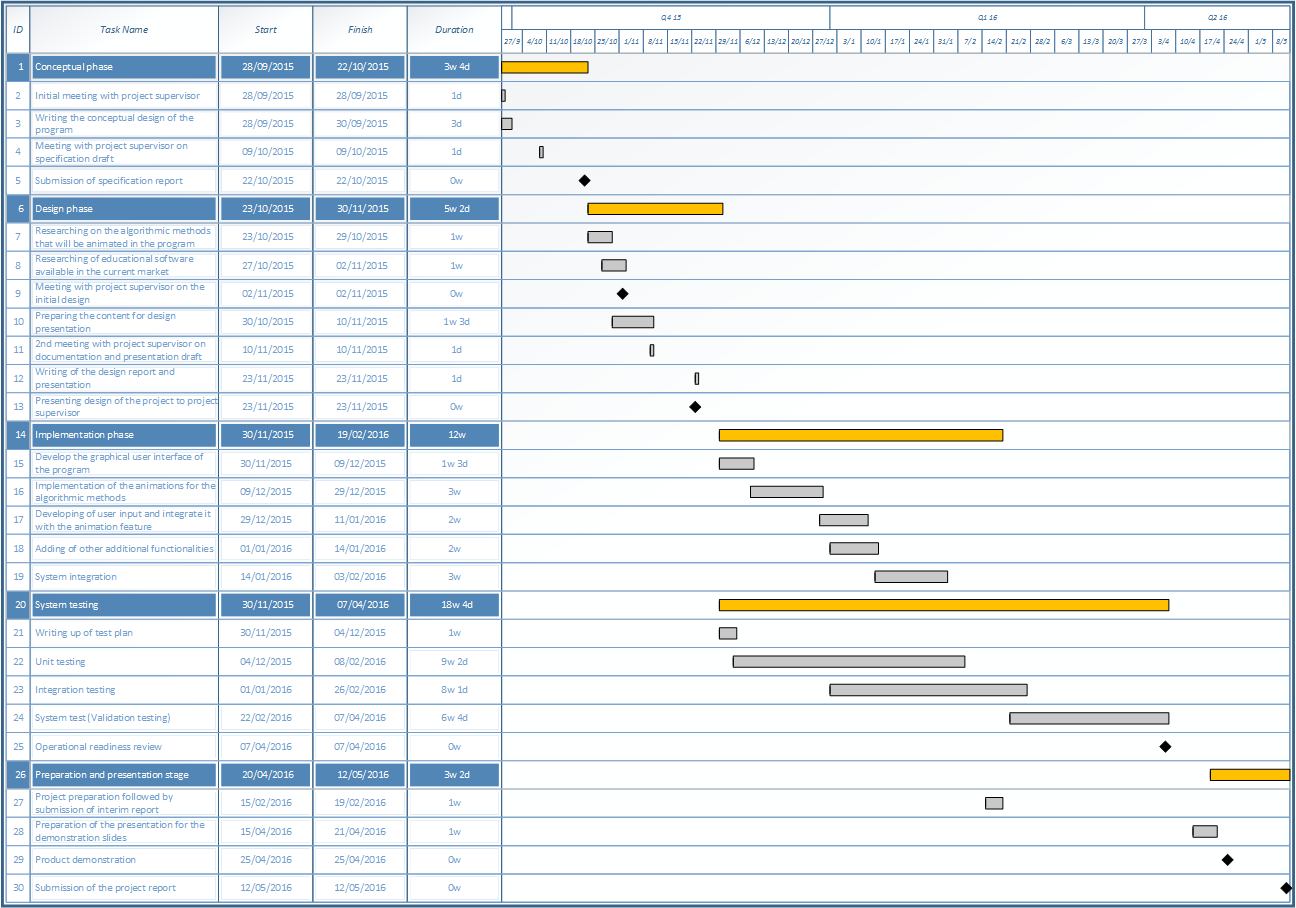
\includegraphics[scale=0.78]{images/report_images/ganttChart.png}
\caption{The updated gantt chart.}
\label{ganttChart}
\end{figure}
\end{landscape}
